\chapter{Final Nutritional Profile of the Bar - Lucas}
\setlength{\headheight}{12.71342pt}
\addtolength{\topmargin}{-0.71342pt}


\section{Nutritional Composition Overview}
In this section of the report, the macronutrient composition of the hemp seed protein bar is examined, namely protein, dietary fibre, and fatty acids. The final nutritional profile was estimated based on the formulation and calculated contributions of each ingredient. Table 6 shows the magnitude of each ingredient in the bar, where the highlighted cells represent the top contributors that will be examined in greater detail. This section further outlines the amino acid and fatty acid spectrum, evaluates potential nutrition and health claims considering EU regulations and EFSA opinions, and compares the bar’s profile to existing market products.

\section{Macronutrient Composition}
As shown in Table 6, the hemp seed protein bar delivers 209.6 kcal per 53.5 g bar, with a macronutrient profile characterised by 12.36 g protein, 4.28 g dietary fibre, 5.84 g fat, 6.27 g moisture, and 24.75 g carbohydrates. This balance between protein, fibre, and healthy fats underlines the bar’s potential as a nutrient-dense snack.

\vspace{1em}
The overall macronutrient profile was calculated using data from various sources to determine the contribution of each ingredient. For each raw material, published nutrient values were combined with the amount used per bar (g) to estimate the contribution of the respective ingredient. The calculations followed Equation 5.1. 


\begin{equation}
    \text{Contribution [g]} = 
    \frac{\text{Nutrient content [g/100g]} \times \text{Ingredient weight [g]}}{100}
    \label{eq:contribution}
\end{equation}

This approach was applied for protein, dietary fibre, fat and moisture. Carbohydrates were excluded from direct analysis, thus their content was derived by calculating the difference, as outlined in Equation 5.2. 

\begin{equation}
    \text{Carbohydrates [g]} = 
    \text{Total weight [g]} - (\text{Protein} + \text{Fat} + \text{Dietary fibre} + \text{Moisture})
    \label{eq:carbohydrates}
\end{equation}

The energy content of the bar was subsequently estimated while adhering to the conversions factors defined in regulation (EU) no. 1169/2011 (protein 4 kcal/g, carbohydrates 4 kcal/g, fibre 2 kcal/g) art\_17. The energy content for moisture was assumed to contribute with 0 kcal/g, thus neglected in the calculations. 

\vspace{1em}
Based on published nutrient values and the calculations described, the bar (53.5 g) provides 209.6 kcal, equivalent to 391.7 kcal/100 g. Its macronutrient composition - 23.1\% protein, 8.0\% dietary fibre, and 10.9\% fat - qualifies the product for the nutrition claims, “High protein” and “High fibre.” These claims comply with the conditions defined in the Annex of Regulation (EC) No 1924/2006, which governs nutrition and health claims across the European Union art\_16.    

\subsection{Protein Content and Quality}
Protein intake is essential for muscle protein synthesis, but the source and type of protein substantially influences its digestibility and utilisation. Since humans cannot synthesise essential amino acids, these must be obtained through diet. Consequently, the overall protein composition, and particularly the essential amino acids profile, is a key to determine protein quality art\_08.

\vspace{1em}
The hemp seed protein bar provides a total of 12.36 g protein per bar. As shown in Table 6, the main contributors for protein are potato protein isolate, rolled oats and dehulled hemp seeds. Dehulling is a processing step which has a significant effect on protein quality. It improves digestibility and reduces antinutritional factors, while also elevating the protein fraction of the hemp seed (hemp\_book). To further characterise the protein profile, Table 3 presents an in-depth analysis of the protein composition, with respect to each ingredient’s amino acid composition. The data was compiled from multiple sources, yet the methodologies used for amino acid determination has been similar across the studies (FridaFood, art\_08, art\_09, art\_10).

\vspace{1em}
The amino acid profile derived from the three main protein contributors includes all nine essential amino acids, confirming the bar as a complete protein source for the consumer. In each of the three main protein contributors, Leucine is the most abundant essential amino acid. Overall, Leucine makes up 5.32\% of the total amino acids contributed by the three ingredients. The combined amount of essential amino acids, derived from these contributors, amounts to 2568.83mg, of which Leucine alone constitutes 22.54\%.

\vspace{1em}
For both rolled oats, and dehulled hemps seeds, the lowest contribution stems from Tryptophan. General consensus, regarding the hemp seed amino acid profile identifies Lysine as the limiting essential amino acid. However, published values vary considerably depending on the analytical methods used, cultivation conditions and cultivar (hemp\_book). 

\vspace{1em}
Conversely, Tryptophan was not identified in published data for potato protein isolate, suggesting a scarce amounts present. For this ingredient, Methionine and Histidine was reported as the limiting essential amino acids, only contributing with 1300 mg/100g, which is substantially lower than the levels of the other essential amino acids. 

\vspace{1em}
The hemp seed protein bar exhibits an overall balanced essential amino acid profile, with only Tryptophan contributing under 1\% of the total amino acids, largely due to the absence of reported values in the potato protein isolate. The combination of the three main protein contributors therefore provides an amino acid profile, that can support several potential health benefits. In dehulled hemp seeds, Leucine, Phenylalanine, and Valine are three most abundant essential amino acids. Of these, only Valine is the only one not shared by the top three essential amino acid contributors in potato protein isolate. 

\vspace{1em}
Valine is one of the branched-chain amino acids (BCAAs), together with Isoleucine and leucine (art\_18). Elevated levels of Valine have been associated with various proposed benefits including improved weight gain, weight gain ratio, enhanced intestinal morphology, strengthened immune responses and increased bone density and strength (art\_19). As an essential amino acid, sufficient dietary intake is important, since valine is directly associated with protein synthesis and functions as a glucogenic amino acid within energy metabolism (art\_19). Although, valine itself has not been authorised any specific health claims under EU law, protein as a whole is recognised by EFSA to contribute to the maintenance and growth of muscle mass (art\_20).

\vspace{1em}
The combination of potato protein isolate, rolled oats, and dehulled hemp seeds enhances the amino acid profile, positioning the hemp protein bar as a sustainable and nutritionally valuable alternative to other conventional protein bars on the market. In addition, the presence of bioactive amino acids supports the bar’s functional value, making hemp a promising ingredient, as a source for high-quality plant protein.

begin{table}[H]
    \centering
    \begin{table}[H]
        \caption{Amino acid composition of the three main protein-contributing ingredients in the hemp seed protein bar (rolled oats, potato protein isolate, and dehulled hemp seeds). The light orange rows indicate essential amino acids (EAAs). Within each amino acid column, the green shading represents relative contribution, ranging from light green (third highest contributor) to dark green (highest contributor). Red cells highlight the lowest contributing ingredient for that specific amino acid.}
    \label{tab:df_amino_acids_01}
    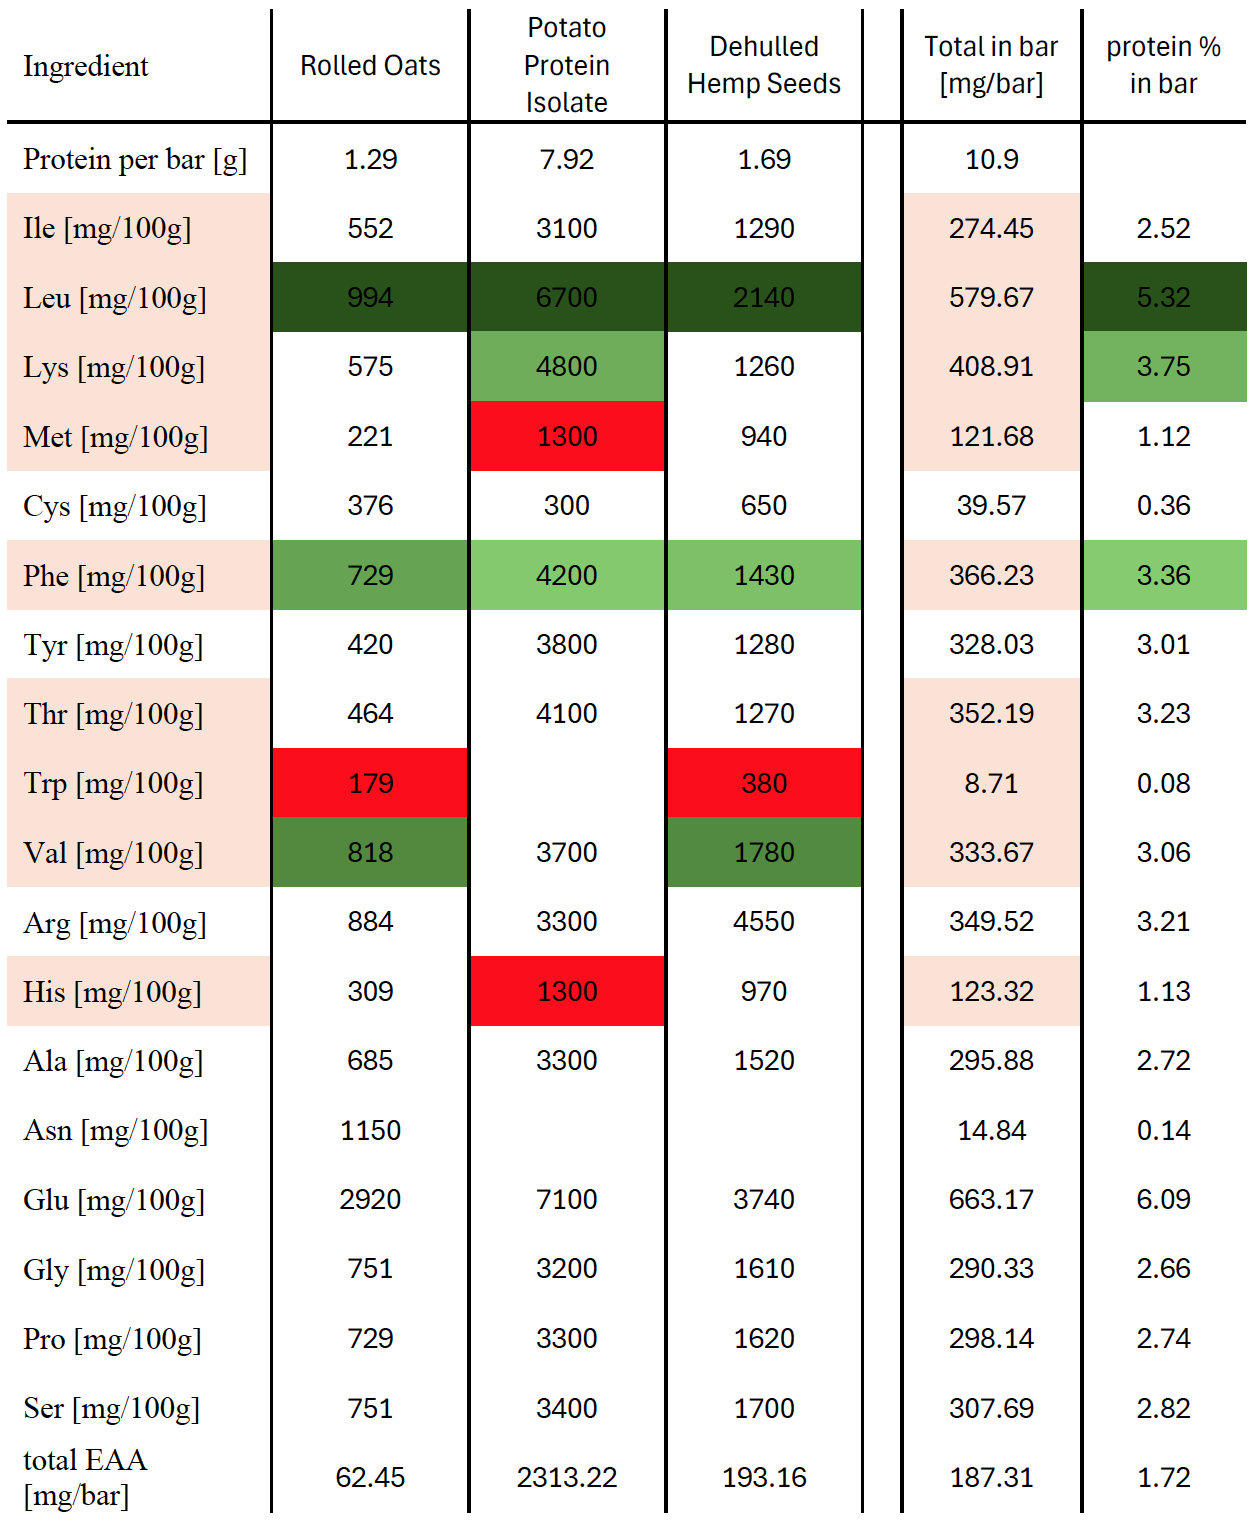
\includegraphics[width=\linewidth]{Figures/tab_amino_acid_01.png}
\end{table}


    
\subsection{Dietary Fibre Content} 
Dietary fibres are carbohydrate polymers that cannot be absorbed in the human small intestine. These polymers, which contains three or more monomer units, have shown positive potential health benefits with significant prospect of improving carbohydrate metabolism and reducing cholesterol levels (art\_12\_01, art13\_02). In addition, certain dietary fibre factions act as prebiotics, and has shown physiological beneficial effects by supporting colonic fermentation and short-chain-fatty acids (art\_13\_02, art\_14). 

\vspace{1em}
The hemp seed protein bar provides a total of 4.28 g dietary fibre per bar. This corresponds to 8 g/100g which exceeds the conditions specified in the Annex of Regulation (EX) No. 1924/2006, for allowing a product to be labelled as “high fibre”.

\vspace{1em}
As shown in Table 6, the main dietary fibre contributors of the hemp seed protein bar are whole hemp seeds, dates (pitted), and rolled oats, who each contributes with 1.32 g, 1.06 g, and 0.99 g, respectively. Processing also influences the dietary fibre profile of the ingredients. In oats, kilning has been used to inactivate lipase enzymes (art\_24), drying dates concentrates their fibre fractions while using whole hemp seeds (un-hulled) preserves their full dietary fibre content. Together, these three ingredients provide the majority of the dietary fibre in the product. When compared with the relative proportions in the product (Table 4), it can be noted, that whole hemp seeds, despite representing only 6.54\% of the bar’s weight, contributes the largest share of the total dietary fibre. Conversely, dates and rolled oats, which consist of 30.84\% and 18.69\% of the bar, respectively, provide less fibre relative to their much larger share of the formulation.

\vspace{1em}
Table 4 contains several blank entries, reflecting that not all ingredients contribute to each of the listed dietary fibre type, and that published data remain scarce, particularly for whole hemp seeds. Nevertheless, it is noteworthy that whole hemp seeds consistently display higher values g/100g for their respective fibre fractions. This highlights the role for whole hemp seeds as the most fibre-dense ingredient and the main contributor to the label “high fibre”. 

\vspace{1em}
The three main ingredients providing dietary fibres, contribute with a diverse palette of fibres. Whole hemp seeds mainly contribute with insoluble fibres such as cellulose, lignin, and hemicellulose. Rolled oats supply cellulose + $\beta-glucan$, lignin, and arabinoxylan, while dates provide these fraction as well as pectin. These fibres differ in solubility and fermentability, thus contributing to a complementary total dietary fibre profile of the hemp seed protein bar (art\_15).

\vspace{1em}
The data used for calculating the fibre fractions for both dates and rolled oats were obtained from published sources given as g/100g dry weight, and g/kg dry weight, respectively. In order to express these values on an as-is basis g/100g, the first step was to make a moisture content correction for the respective ingredients. These conversions were carried out according to Equation 3 and Equation 4, respectively. 


\begin{equation}
    x_{\text{as-is}}\!\left[\frac{\mathrm{g}}{100\,\mathrm{g}}\right]
    = x_{\mathrm{DW}}\!\left[\frac{\mathrm{g}}{100\,\mathrm{g}}\right]\cdot
    \bigl(1 - x_{\text{moisture}}\bigr)
    \label{eq:asis_simple}
\end{equation}

And

\begin{equation}
    x_{\text{as-is}}\!\left[\frac{\mathrm{g}}{100\,\mathrm{g}}\right]
    = \frac{\,x_{\mathrm{DW}}\!\left[\frac{\mathrm{g}}{100\,\mathrm{g}}\right]\,}{10}\,\cdot
    \bigl(1 - x_{\text{moisture}}\bigr)
    \label{eq:asis_div10}
\end{equation}
    
The values for the dietary fibre fractions for whole hemp seeds were given in \% of dry weight, so the calculation had to follow Equation 5.     

\begin{equation}
    x_{\text{as-is}}\!\left[\frac{\mathrm{g}}{100\,\mathrm{g}}\right]
    = \bigl( x_{\mathrm{DW}}\!\left[\tfrac{\mathrm{g}}{100\,\mathrm{g}}\right]
    \cdot (1 - x_{\text{moisture}}) \bigr)
    \cdot x_{\text{DFfraction}}
    \label{eq:asis_dffraction}
    \end{equation}

    These conversions (Equation 3-5) ensured that all reported values, despite differences in study and unit expression, were standardised to a consistent unit. This enabled a direct comparison between the fibre fractions contributed by the three ingredients. 

\begin{table}[H]
    \centering
    \caption{Contribution of the main dietary fibre sources (dates, rolled oats, and whole hemp seeds) to the hemp seed protein bar,
    expressed as total dietary fibre per bar and distribution of fibre fractions. Coloured cells indicate relative contribution, with light
    green representing lowest top three value and dark green representing the highest of the top three. The red coloured cells indicate the
    lowest value for each ingredient.}
    \label{tab:df_tab_01}
    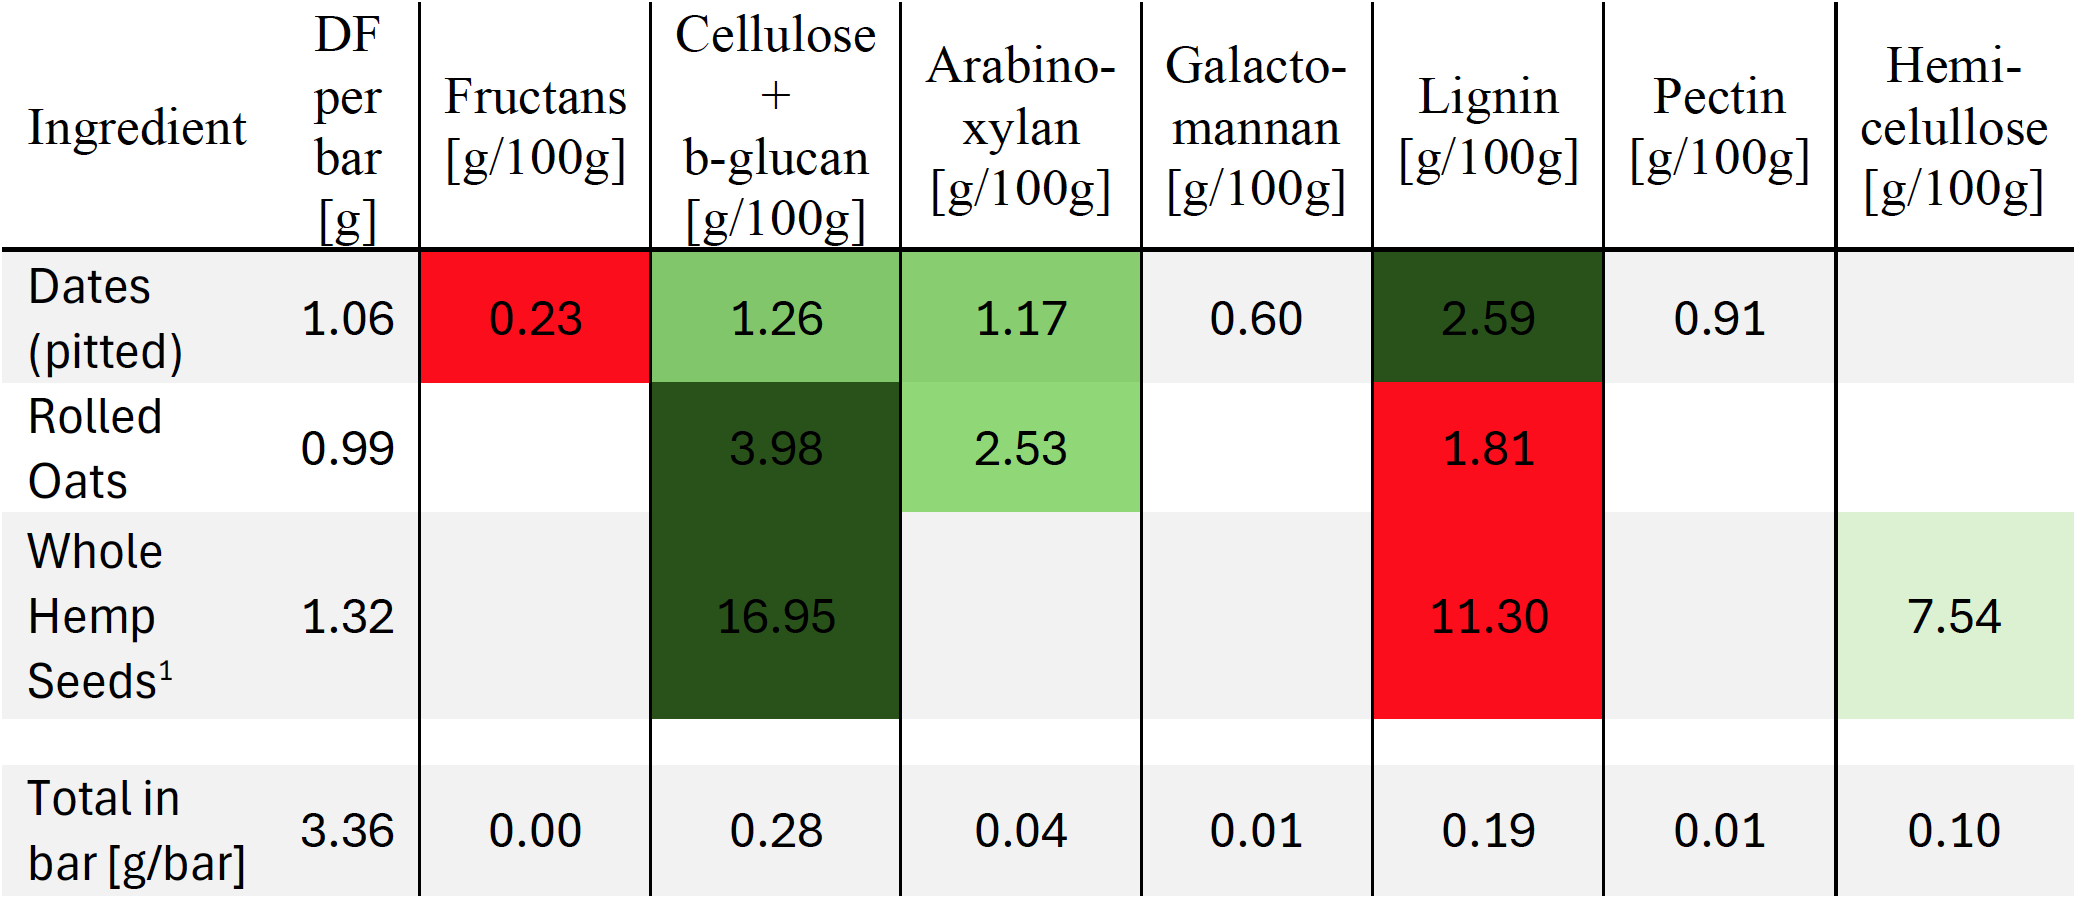
\includegraphics[width=\linewidth]{Figures/tab_df_01.png}
\end{table}

\subsection{Fatty Acid Profile}
The hemp seed protein bar has a total fat content of 5.84 g. The main contributors to this fat content
are dehulled hemp seeds, whole hemp seeds, and rolled oats, which contribute with 3.38 g, 1.09 g,
and 0.69 g, respectively, as shown in Table 6. Processing steps also affect the lipid quality.

\vspace{1em}
Processing steps also affect the lipid quality. Dehulling the hemp seeds increases the fat fraction by removing the hull mass. For a deeper insight into the specific fatty acid profile of the hemp protein bar, Table 5 was constructed to illustrate the distribution of fatty acid fractions from the top three ingredients. 

\vspace{1em}
It can be seen in Table 5, that the fatty acid profile is dominated by the polyunsaturated fatty acids (PUFAs). Notably, linoleic acid (LA, C18:2 n-6) and $\alpha$-linoleic acid (ALA, C18:3 n-3) constitutes 69.47\% of the total fatty acids quantified in the bar. These two essential fatty acids, LA (an omega-6) and ALA (an omega-3), cannot be synthetised by the human body and must therefore be obtained through diet. The abundance in the fatty acid profile highlights the nutritional value of the hemp protein bar. Previous studies have reported that LA and ALA from hemp seeds may the nervous system, supporting the health of blood vessels and to protect against cardiovascular diseases (art\_21). 

\vspace{1em}
Omega-6 tends to have pro-inflammatory pathways, whereas omega-3 supports anti-inflammatory responses. Therefore, maintaining an appropriate balance between these fatty acids is imperative (art\_21). Although EFSA does not prescribe a fixed omega-6 to omega-3 ratio, its Adequate Intake levels for LA (4\% of energy) and ALA (0.5\% of energy) imply a target ratio of approximately 3\:1. The hemp protein bar provides 1.022 g of omega-6 and 0.430 g of omega-3, yielding a ratio of 2.38\:1, close to, but slightly below the recommended guidelines (art\_22). 

\vspace{1em}
As stated, EFSA has set the Adequate Intake levels for LA and ALA to 4E\% and 0.5E\%, respectively. Based on a diet of 2000 kcal, this corresponds to approximately 8.9 g/day of LA and 1.1 g/day of ALA. 

\vspace{1em}
The hemp protein bar will provide roughly 11.5\% and 39\% of the daily requirements of LA and ALA, respectively. Although the substantial contribution to the daily fatty acid intake, these levels does not meet the conditions set by EU for nutrition and health claims. ALA falls below the $geq$ 0.3 g/100kcal threshold for the claim “source of omega-3 fatty acids” (art\_23), and LA remains below the $\geq$ 1.5 g/100kcal threshold requires for the claim “contributes to the maintenance of normal blood cholesterol levels” (art\_24).

\vspace{1em}
Saturated fatty acids (SFAs) in the hemp protein bar sum to 0.277g per bar, or 13.27\% of the total fatty acid profile. Palmitic acid (C16:0) is the predominant fraction, contributing with 0.199 g per bar. 
Monounsaturated fatty acids (MUFAs) account for 0.360 g of the hemp bar, representing 17.24\% of the 2.09 g total fatty acids. Table 5 illustrates that oleic acid (C18:1, n-9) is the dominant MUFA, consistently ranking among the three most abundant fatty acid fractions in dehulled hemp seeds, whole hemp seeds, and rolled oats. 


\begin{table}[H]
    \centering
    \caption{Contribution of the main dietary fibre sources (dates, rolled oats, and whole hemp seeds) to the hemp seed protein bar,
    expressed as total dietary fibre per bar and distribution of fibre fractions. Coloured cells indicate relative contribution, with light
    green representing lowest top three value and dark green representing the highest of the top three. The red coloured cells indicate the
    lowest value for each ingredient.}
    \label{tab:fatty_acid_tab_01}
    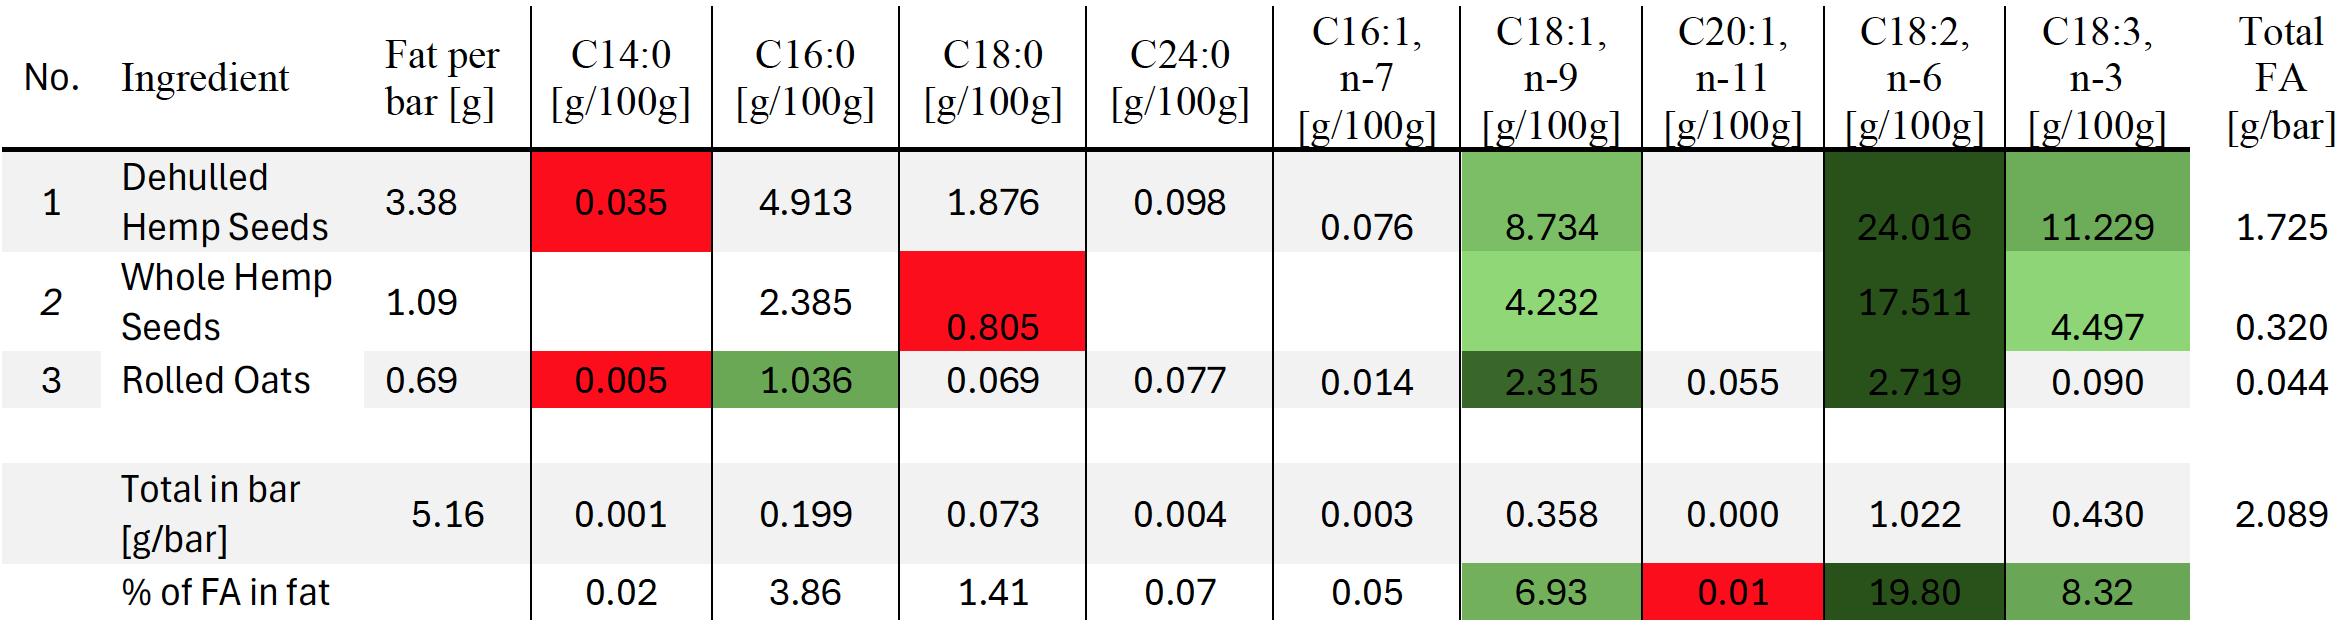
\includegraphics[angle=90,origin=c,width=0.25\textheight]{Figures/tab_fatty_01.png}
\end{table}
